\chapter{Object Reconstruction and Selection}
\label{chap:object_reco}

\newpage

\section{Introduction}

%High-level overview
The CMS $H\rightarrow{\gamma\gamma}$ analysis works by searching for excess production in the distribution of diphoton invariant masses. A Higgs boson signal will manifest as a small bump on top of a continuous distribution due to background processes from Standard Model diphoton production.

The invariant mass of a diphoton system is calculated with the expression
\begin{equation}
    m_{\gamma\gamma} = \sqrt{2E_{\gamma_1}E_{\gamma_2}(1-\cos{\alpha})},
\end{equation}
where $E_{\gamma_1}$ and $E_{\gamma_2}$ are the energies of the leading energy photon and subleading energy photon respectively, and $\alpha$ is the opening angle between them. 
To determine the value of $\alpha$ we require the locations of the photons in the ECAL and the correct originating vertex. 
The CMS ECAL gives a good determination of the photon location in $z$ and $\phi$, but it does not provide any pointing information: to determine $\alpha$ precisely we need to determine the correct vertex by other means.
If the selected vertex is within $1$\,cm of the correct vertex the contribution of spatial uncertainty to the mass resolution is negligible and is dominated by the energy resolution of the ECAL. 
Good identification and measurement of photons and their verices are therefore crucial to the analysis, but there are also other objects used which indicate specific signal production modes and will aid signal extraction.

\section{ECAL Clusters and Particles}

ECAL clusters are used in many of the object of interest in this chapter and are especially important for photons. 
The clustering begins with the identification of local energy maxima above a threshold value, these are referred to as seeds. 
After this topological clusters are grown from the seeds by gathering crystals which share at least one side with a seed, or crystals clustered with a seed, with energy above another threshold which is equal to $2\sigma$ of the ECAL electronic noise (up to 80\,MeV in the barrel and 300\,MeV in the endcaps).
Finally, these clusters are merged to form superclusters which allow for good energy containment, accounting for variation in the construction of the ECAL with $|\eta|$, and pileup robustness.



Physics objects are reconstructed with the CMS global event description known as particle flow (PF). 
PF uses information from all the subdetectors to identify and reconstruct individual particles produced within CMS, and to achieve good energy resolution.
The sorts of nformation used as inputs are tracks from the tracker, tracks from the muon systems, and energy clusters from the ECAL and HCAL. Depending on which of these are present, PF will output `PF candidates' which correspond to different types of semi-stable particles 
\begin{itemize}[leftmargin=.5in,noitemsep]
    \item Photons: ECAL deposition is present with no associated track in tracker. The energy of photons is obtained from the ECAL. 
    \item Electrons: ECAL supercluster is present with associated track in tracker. Energy is determined with electron momentum at the primary vertex, the ECAL deposition, and the energy of associated Bremsstrahlung photons. 
    \item Muons: compatible tracks in tracker and muon system. Energy is determined from the curvature or the tracks. 
    \item Charged Hadrons: track in tracker, ECAL deposition and associated HCAL deposition. Energy is determined from the track curvature, and the matching ECAL/HCAL deposits corrected for effects from zero-supression and for th response of the calorimeters to hadronic showers.
    \item Neutral Hadrons: measured with the corrected energies from the ECAL and HCAL. 
\end{itemize}
These PF candidates are then used to construct jets, and to determine missing transverse momentum $p_{T}^{miss}$.
This process is applied in the same way to data collected with the CMS detector and data from simulation.


\section{Samples}

\subsection{Trigger}
The analysis uses events selected with the two-step CMS triggering system (L1T and HLT). The objective of this system is to keep the event rate below and acceptable level due to limited bandwidth resources whilst keeping signal efficiency a high as possible. Requirements at L1T are looser because it uses fast coarse measurement, HLT uses more stringent requirements to compensate for any inefficiencies from this. 

At L1T we require one or two energy deposits in the ECAL with energy thresholds that varied over the 2016 running period. For the single deposit, energy requirements are more stringent at 25\,GeV during low luminosity up to 40\,GeV at high-luminosity periods to keep the trigger rate to an acceptable level. For two deposits at high-luminosity 22\,Gev and 15\,GeV were required. 

At HLT events were selected with $E_{T}$ thresholds of 30\,GeV and 18\,GeV for the leading and subleading photon respectively. Furthermote, the selection has loose requirements on the shape of the electromagnetic showers, isolation variables, and the ratio of deposition in the ECAL compared to the HCAL. 

These selections have their efficiencies measured with the `tag-and-probe' technique. 
This uses the resonant production and decay to pairs of well-understood particles near their mass peak to ensure a pure and well-understood sample. 
In the $H\rightarrow{\gamma\gamma}$ analysis $Z\rightarrow{}e^{+}e^{-}$ is used as both electrons and photons are reconstructed with the ECAL clustering, so one can use dielectron decays as a proxy for diphotons. 
A strict ID requirement is placed on one of the decay products (the tag) and a looser requirement is placed on the other (the probe). 
The requirement on the probe should be loose enough that it does not affect the selection being measured. The selection efficiency may then be measured as the proportion of the probes which satisfy the selection.
%Ref for tag and probe from the PAS


\subsection{Data}
The data used in the analysis corresponds to the 35.9\,fb$^{-1}$ of proton-proton collision data recorded by the CMS experiment in the 2016 run period with a centre of mass energy of $s=\sqrt{13}$\,TeV and selected with the trigger requirements described above. 



\subsection{Simulation}

Simulated samples are used for a variety of tasks such as to train the ML models of the analysis, to optimise cuts and categorisations, producing signal models, and to perform validations. 

Signal events are simulated for a range of mass points from 120\,GeV to 130\,GeV using cross-sections and branching ratios recommended by the LHC cross-section working group. 
The signal events are generated at next-to-leading order in perturbative QCD with \texttt{MadGraph5_{}aMC@NLO}, with  parton showers and hadronization modelled with \texttt{pythia8}. The \texttt{pythia} tune parameter set \texttt{CUETP8M1} is used.

The background simulations are generated in different ways. For the main irreducible background from prompt diphotons \texttt{Sherpa} is used which includes Born processes with up to three jets as well as box diagram processes at leading order. 
For the $\gamma$-jet and jet-jet reducible backgrounds where jets are mistakenly reconstructed as photons we use \texttt{pythia8} with a filter applied to enhance the electromagnetic energy content of the jets. 
Finally, samples for validation $W\gamma$ and $Z\gamma$ are simulated with \texttt{Madgraph} and Drell-Yan (DY) is simulated with \texttt{Madgraph_{}aMC@NLO}


The CMS detector itself is simulated in detail with \texttt{GEANT4}. 
This includes the simulation of both in-time and out-of-time pileup. 
Simulated events are then weighted such that they reproduce the pileup distribution observed in data from CMS.


\section{Photon Reconstruction}
Photons are reconstructed from calibrated ECAL superclusters which have had corrections calculated with a collection of techniques. One of these is a BDT regressor applied to account for detector effects. The resulting candidate photons are then put through a preselection aimed at rejecting non-prompt photons due to jet fragments, this also uses the output of a BDT classifier as a selection criterion.
All of these steps, including their validation, use a common collection of variables which will be detailed in the next subsection for later reference. 

\subsection{Common Variables}
The set of common variables can be divided into three types: shower shape variables and isolation variables. 
Shower shape variables describe properties of the electromagnetic showers within the ECAL which will allow us to infer information about the object. For example, whether a shower is from a pristine or a pair-converted photon
The set of shower shape variables consists of the following:
\begin{itemize}[leftmargin=.5in,noitemsep]
    \item $R_{9}$, the energy deposited in a $3\times{}3$ array of crystals around the most energetic crystal in a supercluster divided by the total energy in the supercluster. Low values indicate a photon that has undergone pair conversion and its energy is spread over a larger area. 
    \item $S_4$, the energy of the $2\times{}2$ grid which contains the seed crystal divided by the total SC energy.
    \item $n_{\mathrm{clusters}}$, number of clusters in the supercluster.
    \item $\sigma_{\eta}$, the standard deviation of the log-energy-weighted $\eta$ of the SC crystals.
    \item $\sigma_{\phi}$, the standard deviation of the log-energy-weighted $\phi$ of the SC crystals.
    \item $\sigma_{rr}$, shower width in the $r$ direction in the CMS transverse plane.
    \item $cov_{\eta\phi}$, covariance between the locations in $\eta$ and $\phi$ for single crystals centred around the most energetic crystal in the supercluster.
    \item $E_{\mathrm{seed}}/E_{SC}$, ratio of seed crystal energy to SC energy
    \item $E_{\mathrm{seed}}/E_{3\times{}3}$, ratio of seed crystal energy to the $3\times{}3$ grid around it
    \item $E_{\mathrm{seed}}/E_{5\times{}5}$, ratio of seed crystal energy to the $5\times{}5$ grid around it
    \item $H/E$, ratio of the deposition in the HCAL to the ECAL around the location of the supercluster
\end{itemize}


Isolation variables measure how well-separated an object, in this case a photon, is from other objects in the event such as electrons or charged hadrons which could imitate the true signal. The set of isolation variables consists of the following
\begin{itemize}[leftmargin=.5in,noitemsep]
    \item $\mathcal{I}_{\gamma}$, photon isolation, the sum of the transverse energy of the particles identified as photons in a cone of $R=0.3$ around the candidate photon.
    \item $\mathcal{I}_{\mathrm{CH}}$, charged hadron isolation, the sum of transverse momenta of charged particles in a $R=0.3$ cone around the candidate photon. 
    \item $\mathcal{I}_{\mathrm{T}}$, track isolation, the sum of transverse momenta of tracks in a hollow cone between $R=0.3$ and $R=0.04$ around the candidate photon.
\end{itemize}



\subsection{Photon Energy Corrections}

The photon energy has a set of corrections applied depending on whether the photon is from simulation or data: individual photon energy correction, an overall energy scale correction in data, and a smearing of the simulated data to match its distribution to data. 

\subsubsection{Photon Energy Correction}
The photon energy correction is computed with a regressor BDT whose target is the ratio of true energy to the raw measured energy of the associated supercluster. It also computes the median uncertainty of the energy. 
The inputs to the BDT are a collection of shower shape variables, position variables, infomation from the preshower subdetector, and pileup-sensitive event-level variables.
The BDT is then trained on simulated photons with two separately trained BDTs in the barrel and endcap regions. 


\subsubsection{Energy Scale}
Once we have the corrected energies, the overall energy scale needs to be corrected to account for detector effects. 
During operation the CMS ECAL recieves large doses of radiation that can degrade its performance over time. 
This will lead to drifts and jumps in the detector response as conditions change, and as a result the measured energy will also drift and jump. 
Scale factors to account for this effect in data are calculated using the $Z\rightarrow{}e^{+}e^{-}$ decay as a standard candle where the electrons are reconstructed as photons. 
Using comparison to simulation, and the well-known value of the $Z$ boson mass, scales are derived for different times and detector locations to bring the measured value of real $Z$ bosons back to the true value. 


\subsubsection{Resolution Smearing}
Simulation also needs to be corrected by comparison to data to make it more realistic. The photon energy resolution in simulated events has a Gaussian smearing added to it which is derived from comparing the width of the $Z\rightarrow{}e^{+}e^{-}$ mass distribution in different categories depending on $|\eta|$-location within the detector (two in the barrel either side of $|\eta|=1$ and two in the endcaps either side of $|\eta|=2$), and the $R_{9}$ variable which measures photon quality (above or below $R_{9}=0.94$).
The mass peak in two of these bins is shown in Figure \ref{fig:object_reco:invariant_mass_validation}.
\begin{figure}[h!]
    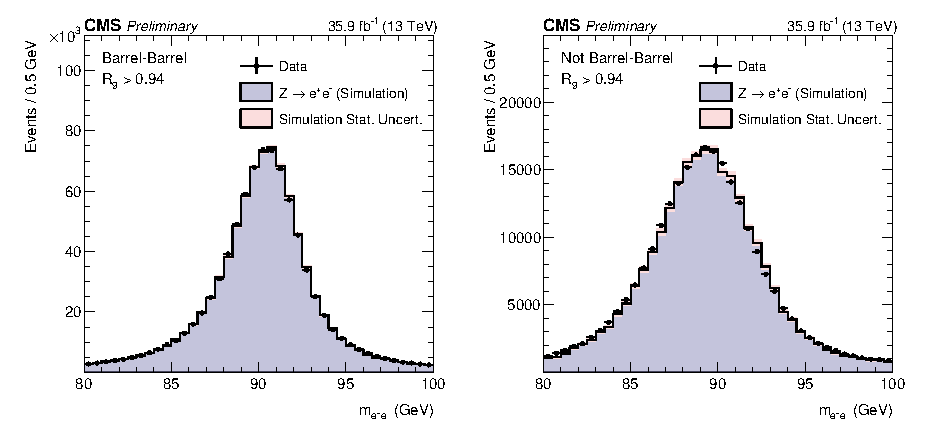
\includegraphics[width=0.95\textwidth]{figures/object_reco/CMS-PAS-HIG-16-040_Figure_001.pdf}
    \caption{A comparison between data and simulation of dielectron invariant mass}
        \label{fig:object_reco:invariant_mass_validation}
\end{figure}

\subsection{Photon Preselection}
%intro
Before a photon can enter the analysis it must pass a set of selection criteria, the photon preselection, which are slightly more stringent than the trigger and vary by location. First photons are grouped into diphotons by considering all possible pairs in the event, then the criteria are applied (with the exception of $p_{T}$ cuts) on a per-photon basis.
The criteria are:
%List of requirements
\begin{itemize}[leftmargin=.5in,noitemsep]
    \item Electron veto: rejection if there is a track associated to the supercluster.
    \item Photon $p_{T}$s: $p_{T}^{\gamma_1} > 30$\,GeV and $p_{T}^{\gamma_2} > 20$\,GeV
    \item $R_{9}$: is not used to reject events outright, but determines which other selections are applied. If $R_{9} < 0.85$ in the barrel or $R_{9} < 0.9$ in the endcaps additional requirements are imposed. 
    \item Energy-weighted $\eta$ width: $\sigma_{\eta\eta} < 0.015$ in the barrel and $\sigma_{\eta\eta} < 0.015$ in the endcaps
    \item HCAL/ECAL deposition: $H/E < 0.08$ in all regions.
    \item Photon isolation: $\mathcal{I}_{\gamma} < 4.0$ in all regions. 
    \item Track isolation: $\mathcal{I}_{T} < 6.0$ in all regions.
    \item Charged hadron isolation: $\mathcal{I}_{CH} < 20$\,GeV.
    \item Photon ID: score from a BDT classifier that discriminates between prompt photons and jet fragments.
\end{itemize}
Both photons must also satisfy either of two additional requirements:
\begin{itemize}[leftmargin=.5in,noitemsep]
    \item $R_{9} > 0.8$ and $\mathcal{I}_{CH} < 20$\,GeV
    \item $\mathcal{I}_{CH}/p_{T}^{\gamma} < 0.3$
\end{itemize}

%Schema table of thesholds
The efficiency of these criteria are measured using $Z\rightarrow{}e^{+}e^{-}$ and the tag-and-probe method, 
with the exception of the electron veto which uses $Z\rightarrow{}\mu^{+}\mu^{-}\gamma$. The preselection efficiencies are summaried in Table \ref{tab:object_reco:presel_eff}
%Table of efficiencies
\begin{table}[h!]
    \begin{tabular}{ l | c | c | c }
        Preselection Category& $\epsilon_{\mathrm{data}} (\%)$ & $\epsilon_{\mathrm{sim}} (\%)$ & $\epsilon_{\mathrm{data}}/\epsilon_{\mathrm{sim}}$ \\
        \hline
        Barrel, $R_{9}>0.85$ & $94.2\pm0.9$ & $94.7\pm0.9$ & $0.995\pm0.001$ \\
        Barrel, $R_{9}<0.85$ & $82.5\pm0.7$ & $82.5\pm0.7$ & $1.000\pm0.003$ \\ 
        \hline
        Endcap, $R_{9}>0.85$ & $90.1\pm0.2$ & $91.3\pm0.1$ & $0.987\pm0.005$ \\ 
        Endcap, $R_{9}<0.85$ & $49.7\pm1.4$ & $53.8\pm1.5$ & $0.923\pm0.010$ \\ 
\end{tabular}
    \caption{Preselection efficiencies}
    \label{tab:object_reco:presel_eff}
\end{table}





\subsection{Photon Identification}
%Intro
The photon identification BDT is a classifier whose task is to discriminate between real prompt photons and photon-like jet fragments which satisfy the preselection criteria. 
The BDT is trained using simulated $\gamma + $jet events where the reconstructed photons are matched to a generator-level particle, if there is no match it is considered to be in the non-prompt class.
To avoid the BDT introducing a dependence on on photon kinematics the signal photons are reweighted such that their distribution in $p_{T}$ and $\eta$ is flat. 
The classifier recieves the following input features:
%variables
\begin{itemize}[leftmargin=.5in,noitemsep]
    \item Shower shape variables: $\sigma_{\eta}$,$\sigma_{\phi}$,$\sigma_{RR}$,$\sigma_{\eta\eta}$,
    \item Isolation variables: $\mathcal{I}_{\gamma}$, $\mathcal{I}_{CH}^{SV}$ the charged hadron isolation for the selected vertex, and $\mathcal{I}_{CH}^{WV}$ the charged hadron isolation for the wrong vertex 
    \item Other variables: $\rho$, the median energy density per unit area of the event to reduce pileup effects, the $\eta$ location of the SC $\eta_{SC}$, and the energy of the $E_{SC}$. 
\end{itemize}

validation plots
\begin{figure}[h!]
    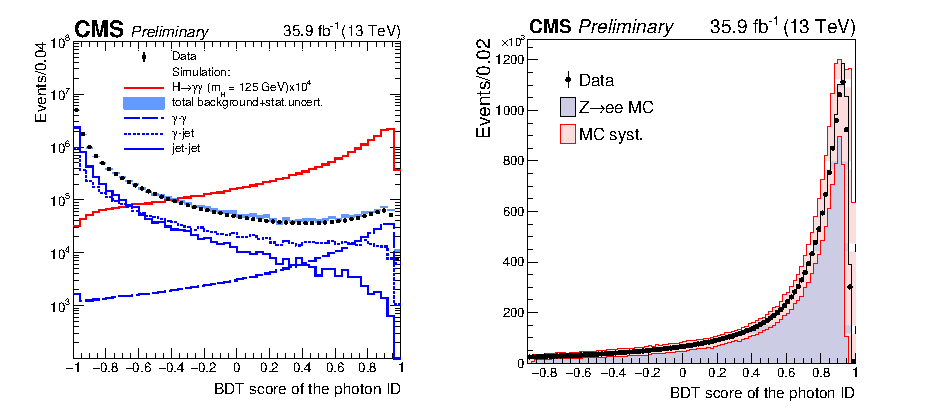
\includegraphics[width=0.95\textwidth]{figures/object_reco/CMS-PAS-HIG-16-040_Figure_002.pdf}
    \caption{Photon ID BDT validation}
        \label{fig:object_reco:photon_id_bdt}
\end{figure}


systematics

\section{Vertex Reconstruction}
How to find vertices: charged tracks

\subsection{Vertex Selection}
Yet another BDT to find the vertex with tracks

\subsection{Vertex Probability}
another for prob it's right


\section{Other Objects}

\subsection{Electrons}

\subsection{Muons}

\subsection{Jets}
